\chapter{Některé příkazy balíčku \texttt{thesis}}

\section{Příkazy pro sazbu veličin a jednotek}

\begin{table}[!h]
  \caption{Přehled příkazů pro matematické prostředí }
  \begin{center}
  	\small
	  \begin{tabular}{|c|c|c|c|}
	    \hline
	    Příkaz    						& Příklad 					& Zdroj příkladu  							& Význam  \\
	    \hline\hline
	    \verb|\textind{...}|	& $\beta_\textind{max}$ 	& \verb|$\beta_\textind{max}$|	& textový index \\
	    \hline
	    \verb|\konst{...}| 		& $\konst{U}_\textind{in}$ 				& \verb|$\konst{U}_\textind{in}$|		& konstantní veličina \\
	    \hline
	    \verb|\prom{...}| 		& $\prom{u}_\textind{in}$ & \verb|$\prom{u}_\textind{in}$| & proměnná veličina \\
	    \hline
	    \verb|\komplex{...}| 	& $\komplex{u}_\textind{in}$ & \verb|$\komplex{u}_\textind{in}$| & komplexní veličina \\
	    \hline
	    \verb|\vekt{...}| 		& $\vekt{y}$ 						& \verb|$\vekt{y}$| & vektor \\
	    \hline
	    \verb|\matice{...}| 	& $\matice{Z}$ 						& \verb|$\matice{Z}$| & matice \\
	    \hline
	    \verb|\jedn{...}| 		& $\jedn{kV}$ 						& \verb|$\jedn{kV}$|\quad či\ \, \verb|\jedn{kV}| & jednotka \\
	    \hline
	  \end{tabular}
  \end{center}
\end{table}



%\newpage
\section{Příkazy pro sazbu symbolů}

\begin{itemize}
  \item
    \verb|\E|, \verb|\eul| -- sazba Eulerova čísla: $\eul$,
  \item
    \verb|\J|, \verb|\jmag|, \verb|\I|, \verb|\imag| -- sazba imaginární jednotky: $\jmag$, $\imag$,
  \item
    \verb|\dif| -- sazba diferenciálu: $\dif$,
  \item
    \verb|\sinc| -- sazba funkce: $\sinc$.
  \item
    \verb|\mikro| -- sazba symbolu mikro stojatým písmem\footnote{znak pochází z~balíčku \texttt{textcomp}}: $\mikro$.

\end{itemize}
%
Všechny symboly jsou určeny pro matematický mód, vyjma \verb|\mikro|, jenž je\\ použitelný rovněž v~textovém módu.






\chapter{Druhá příloha}

\begin{figure}[!h]
  \begin{center}
    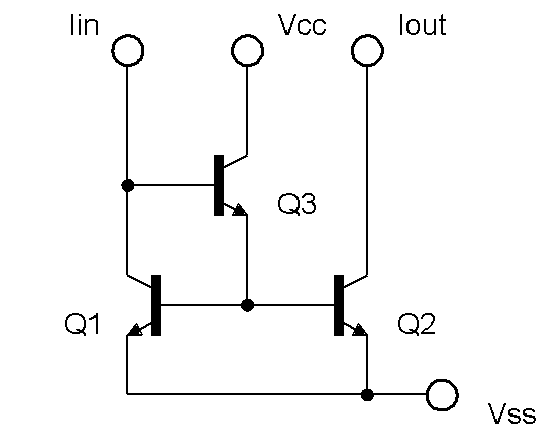
\includegraphics[scale=0.5]{obrazky/ZlepseneWilsonovoZrcadloNPN}
  \end{center}
  \caption{Zlepšené Wilsonovo proudové zrcadlo.}
\end{figure}

Pro sazbu vektorových obrázků přímo v~\LaTeX{}u je možné doporučit balíček \href{https://www.ctan.org/pkg/pgf}{\texttt{TikZ}}.
Příklady sazby je možné najít na \href{http://www.texample.net/tikz/examples/}{\TeX{}ample}.
Pro vyzkoušení je možné použít programy QTikz nebo TikzEdt.




\chapter{Příklad sazby zdrojových kódů}

\section{Balíček \texttt{listings}}

Pro vysázení zdrojových souborů je možné použít balíček \href{https://www.ctan.org/pkg/listings}{\texttt{listings}}.
Balíček zavádí nové prostředí \texttt{lstlisting} pro sazbu zdrojových kódů, jako například:
%
\begin{lstlisting}[language={[LaTeX]TeX}]
\section{Balíček lstlistings}
Pro vysázení zdrojových souborů je možné použít
	balíček \href{https://www.ctan.org/pkg/listings}%
	{\texttt{listings}}.
Balíček zavádí nové prostředí \texttt{lstlisting} pro
	sazbu zdrojových kódů.
\end{lstlisting}
%
Podporuje množství programovacích jazyků.
Kód k~vysázení může být načítán přímo ze zdrojových souborů.
Umožňuje vkládat čísla řádků nebo vypisovat jen vybrané úseky kódu.
Např.:

\noindent
Zkratky jsou sázeny v~prostředí \texttt{seznamzkratek}:
\label{lst:zkratky}
\lstinputlisting[language={[LaTeX]TeX},nolol,numbers=left,firstline=1,lastline=1]{text/zkratky.tex}
%
Šířka textu druhého parametru \verb|KolikMista| udává šířku prvního sloupce se zkratkami.
Proto by měla být zadávána nejdelší zkratka nebo symbol.

\iflanguage{czech}{\shorthandoff{-}}{}
%\iflanguage{slovak}{\shorthandoff{-}}{}
\lstinputlisting[language={[LaTeX]TeX},frame=single,caption={Ukázka sazby zkratek},label=lst:symfvz,numbers=left,linerange={bsymfvz-\%\%\%\ esymfvz},includerangemarker=false]{text/zkratky.tex}
%\iflanguage{slovak}{\shorthandon{-}}{}
\iflanguage{czech}{\shorthandon{-}}{}

\noindent
Ukončení seznamu je provedeno ukončením prostředí:
\lstinputlisting[language={[LaTeX]TeX},nolol,numbers=left,firstnumber=22,linerange=22]{text/zkratky.tex}

\vspace{\fill}

\noindent
{\bf Poznámka k~výpisům s~použitím volby jazyka \verb|czech| nebo \verb|slovak|:}\newline
Pokud Váš zdrojový kód obsahuje znak spojovníku \verb|-|, pak překlad může skončit chybou.
Ta je způsobená tím, že znak \verb|-| je v~českém nebo slovenském nastavení balíčku \verb|babel| tzv.\ aktivním znakem.
Přepněte znak \verb|-| na neaktivní příkazem \verb|\shorthandoff{-}| těsně před výpisem a hned za ním jej vraťte na aktivní příkazem \verb|\shorthandon{-}|.
Podobně jako to je ukázáno ve zdrojovém kódu šablony.


\clearpage

%\section{Výpis kódu prostředí Matlab}
Na výpisu nenaleznete příklad kódu pro Matlab, na výpisu \ref{lst:priklad.vypis.kodu.C} zase pro jazyk~C.

\lstnewenvironment{matlab}[1][]{%
\iflanguage{czech}{\shorthandoff{-}}{}%
\iflanguage{slovak}{\shorthandoff{-}}{}%
\lstset{language=Matlab,numbers=left,#1}%
}{%
\iflanguage{slovak}{\shorthandon{-}}{}%
\iflanguage{czech}{\shorthandon{-}}{}%
}



\noindent
\begin{minipage}{\linewidth}


%\section{Výpis kódu jazyka C}

\begin{lstlisting}[frame=single,numbers=right,caption={Příklad implementace první kanonické formy v~jazyce C.},label=lst:priklad.vypis.kodu.C,basicstyle=\ttfamily\small, keywordstyle=\color{black}\bfseries\underbar,]
// první kanonická forma
short fxdf2t( short coef[][5], short sample)
{
	static int v1[SECTIONS] = {0,0},v2[SECTIONS] = {0,0};
	int x, y, accu;
	short k;

	x = sample;
	for( k = 0; k < SECTIONS; k++){
		accu = v1[k] >> 1;
		y = _sadd( accu, _smpy( coef[k][0], x));
		y = _sshl(y, 1) >> 16;

		accu = v2[k] >> 1;
		accu = _sadd( accu, _smpy( coef[k][1], x));
		accu = _sadd( accu, _smpy( coef[k][2], y));
		v1[k] = _sshl( accu, 1);

		accu = _smpy( coef[k][3], x);
		accu = _sadd( accu, _smpy( coef[k][4], y));
		v2[k] = _sshl( accu, 1);

		x = y;
	}
	return( y);
}
\end{lstlisting}
\end{minipage}







\chapter{Obsah přiloženého CD}
Nezapomeňte uvést, co čtenář najde na přiloženém médiu.
Je vhodné okomentovat obsah každého adresáře, specifikovat, který soubor obsahuje důležitá nastavení, který soubor je určen ke spuštění atd.
Také je dobře napsat, v~jaké verzi software byl kód testován (např.\ Matlab 2010b).

Pokud je souborů hodně a jsou organizovány ve více složkách,  je možné pro výpis adresářové struktury použít balíček \href{https://www.ctan.org/pkg/dirtree}{\texttt{dirtree}}.

{\small
%
\dirtree{%.
.1 /\DTcomment{kořenový adresář přiloženého CD}.
.2 loga\DTcomment{loga školy a fakulty}.
.3 FEKT-spec-color.eps.
.3 FEKT-spec-color.pdf.
.3 logolink-op\_vavpi.png.
.3 RE-spec-color.eps.
.3 RE-spec-color.pdf.
.3 SIX\_logo\_zahlavi.png.
.2 obrazky\DTcomment{ostatní obrázky}.
.3 soucastky.eps.
.3 soucastky.png.
.3 spoje.eps.
.3 spoje.png.
.3 ZlepseneWilsonovoZrcadloNPN.eps.
.3 ZlepseneWilsonovoZrcadloNPN.png.
.3 ZlepseneWilsonovoZrcadloPNP.eps.
.3 ZlepseneWilsonovoZrcadloPNP.png.
.2 pdf\DTcomment{pdf stránky generované informačním systémem}.
.3 student-desky.pdf.
.3 student-titulka.pdf.
.3 student-zadani.pdf.
.2 text\DTcomment{zdrojové textové soubory}.
.3 literatura.tex.
.3 prilohy.tex.
.3 reseni.tex.
.3 uvod.tex.
.3 vysledky.tex.
.3 zaver.tex.
.3 zkratky.tex.
.2 navod-sablona\_FEKT.pdf\DTcomment{návod na používání šablony}.
.2 obhajoba.tex\DTcomment{hlavní soubor pro sazbu prezentace k~obhajobě}.
.2 readme.txt\DTcomment{soubor s~popisem obsahu CD}.
.2 sablona.tex\DTcomment{hlavní soubor pro sazbu kvalifikační práce}.
.2 thesis.sty\DTcomment{balíček pro sazbu kvalifikačních prací}.
}
}